\documentclass[letterpaper,10pt]{article}

\usepackage{titling}
\usepackage{listings}
\usepackage{url}
\usepackage{setspace}
\usepackage{subfig}
\usepackage{sectsty}
\usepackage{pdfpages}
\usepackage{colortbl}
\usepackage{multirow}
\usepackage{multicol}
\usepackage{relsize}
\usepackage{amsmath}
\usepackage{wasysym}
\usepackage{fancyvrb}
\usepackage{amssymb}
\usepackage{ifsym}
\usepackage{amsmath,amssymb,amsthm,graphicx,xspace}
\usepackage[titlenotnumbered,noend,noline]{algorithm2e}
\usepackage[compact]{titlesec}
\usepackage{XCharter}
\usepackage[T1]{fontenc}
\usepackage{tikz}
\usetikzlibrary{arrows,automata,shapes,trees,matrix,chains,scopes,positioning,calc}
\tikzstyle{block} = [rectangle, draw, fill=blue!20, 
    text width=2.5em, text centered, rounded corners, minimum height=2em]
\tikzstyle{bw} = [rectangle, draw, fill=blue!20, 
    text width=4em, text centered, rounded corners, minimum height=2em]

\definecolor{namerow}{cmyk}{.40,.40,.40,.40}
\definecolor{namecol}{cmyk}{.40,.40,.40,.40}

\let\LaTeXtitle\title
\renewcommand{\title}[1]{\LaTeXtitle{\textsf{#1}}}


\newcommand{\handout}[5]{
  \noindent
  \begin{center}
  \framebox{
    \vbox{
      \hbox to 5.78in { {\bf ECE356: Database Systems } \hfill #2 }
      \vspace{4mm}
      \hbox to 5.78in { {\Large \hfill #4  \hfill} }
      \vspace{2mm}
      \hbox to 5.78in { {\em #3 \hfill} }
    }
  }
  \end{center}
  \vspace*{4mm}
}

\newcommand{\lecture}[3]{\handout{#1}{#2}{#3}{Lecture #1}}
\newcommand{\tuple}[1]{\ensuremath{\left\langle #1 \right\rangle}\xspace}

\addtolength{\oddsidemargin}{-1.000in}
\addtolength{\evensidemargin}{-0.500in}
\addtolength{\textwidth}{2.0in}
\addtolength{\topmargin}{-1.000in}
\addtolength{\textheight}{1.75in}
\addtolength{\parskip}{\baselineskip}
\setlength{\parindent}{0in}
\renewcommand{\baselinestretch}{1.5}
\newcommand{\term}{Winter 2018}

\singlespace


\begin{document}

\lecture{ 2 --- (Entity-)Relational Model }{\term}{Jeff Zarnett}

\section*{Database Data Models} 
There is a certain level of abstraction provided by the database; that is, the users, even application programmers, may not need to be aware of the way in which the data is stored or handled. With that in mind, there will be a \textit{data model} -- the abstraction that describes the structure of the database~\cite{fds}. The data model is not only how the database is structured in terms of its schema, but also defines some basic operations to access and modify data (and the schema). 

According to~\cite{dsc} there are four rough categories for data models. For the most part we will focus on the first one, the Relational Model. We will also give some consideration to the Entity-Relational model. The other two, Object-Based and Semistructured, will be noted for completeness but are not the focus of much discussion.


\paragraph{Relational Model.} The relational model uses tables to represent data (and there are also tables that contain the relations between those tables). Tables have unique names, and are composed of columns (and column names must be unique per table). An entry in such a table is a row. This is a record-based model in that each table comprises fixed format records of specific types. A record definition says what fields exist and their types (and we have seen that already). Each column in the table is one of the fields~\cite{dsc}.


\paragraph{Entity-Relationship Model.} The entity-relationship model (sometimes abbreviated E-R or ER) model takes the idea of structured types, like a \texttt{struct} in C. Entities have various properties and there are also relationships. Entities are like objects in an object-oriented programming language in that they are supposed to correspond to a cohesive ``thing'' with properties~\cite{dsc}.

\paragraph{Object-Based Data Model.} This model borrows from Object-Oriented Programming to expand it to include the ideas of encapsulation, methods, and object identity, to build on the entity-relationship model~\cite{dsc}.

\paragraph{Semistructured Data Model.} The semi-strutted model is somewhat more flexible than various other models because the attributes may vary. XML is a good example of a semistructured data model. In XML we can easily have a type where things are arbitrary length and types of attributes may vary. 

\section*{Entities and Relationships}

We have already discussed the idea of entities as objects. A vehicle has a VIN, a year, a model, a colour, et cetera. Every vehicle has those attributes, and some of them will be unique (e.g., VIN) to one vehicle and others will be shared (e.g., Volkswagen makes something like 1~000~000 Golf model vehicles in a year). 

In addition to this, we have the concept of a relationship between identities: a vehicle is owned by a person. This is a simple association. The definition of our associations can also contain some important ``rules'' about our data. For example, a vehicle may have only one owner.

To speak more formally about entity relationships we will use some mathematical notation (mostly set notation). The relational model traces its way back to a paper published in 1970 that described the database in mathematical relationships and first-order logic~\cite{codd}. The math may seem intimidating when we first examine it, but ultimately provides an unambiguous and concise way of describing how it all works, even if you don't necessarily adopt that as a way of thinking about the problem. The mathematical description is embodied in a table. 

We need to spend some more time to define some terminology, specifically: domain, tuple, attribute, and relation.  

A \textit{domain} $D$ is a set of atomic values, where atomic means that the value is not divisible in the relational model~\cite{fds}. A telephone number like {(212)~867-5309} may be divisible in the sense that we can identify 212 as the area code, but as far as the database is concerned if a phone number is ten digits it will consider that ten digit phone number to be indivisible. If the database designer intends for area codes to be separate from the remaining digits of the phone number that is a design choice and there will accordingly be two separate fields for it. 

As we already saw in the previous examples about vehicles that fields, domains, have a data type associated with them such as integer, string, et cetera. Oftentimes there is a specified length of the field, such as limiting a phone number to 10 characters. 

To indicate that a value is missing, unknown, or not relevant, there is the possibility for a domain to be \texttt{null}. This is a member of every domain by default, although it is possible to specify that a null is not permitted in the format. The use of null can occasionally cause us some headaches in the same way that null being used as a sentinel value in Java, for example, can lead us to a \texttt{NullPointerException}. One example of the way that null causes problems is that null does not equal null... 

In some terminology that might be slightly confusing, a row in a table represents a \textit{relationship} between a set of values: that is to say that things like ``Volkswagen'' and ``Golf'' and ``2015'' all go together. This is what we call a \textit{tuple}, which corresponds mathematically with an \textit{n-tuple} (that is a tuple with n values in it)~\cite{dsc}. 

The table itself we call a \textit{relation} (which is why this is the ``relational'' model). An \textit{attribute} is then a column in that table. So if the relation is an address, the attributes will be name, street, city, province, postal code... 

Let's recap this mathematically, as in~\cite{fds}: A relation schema $R$ is denoted as $R(A_{1}, A_{2}, ..., A_{n})$. It is named $R$ and has a list of attributes $A_{1}$ through $A_{n}$. Each attribute is the name of a domain $D$. The degree of the relation is the number of attributes. This is the table definition, just explained in a mathematical way.

The table content, or the relation itself, is denoted $r(R)$ and it is the set of n-tuples where $r = \{t_{1}, t_{2}, ..., t_{m}\}$. Each n-tuple is an ordered list of values where each value $v_{i}$ is an element of the domain of attribute $A_{i}$ or the null value. We might reference these as $t[A_{i}]$, $t.A_{i}$, or $t[i]$. 

So if our relation schema $R$ is as follows:
\begin{center}
		\textbf{OWNER\_ADDRESS}\\
	\begin{tabular}{|l|l|}\hline
		\textbf{id} & \texttt{integer not null,  primary key}\\ \hline
		\textbf{name} & \texttt{string(64) not null}\\ \hline
		\textbf{street} & \texttt{string(64) not null}\\ \hline
		\textbf{city} & \texttt{string(32) not null}\\ \hline
		\textbf{province} & \texttt{string(2) not null}\\ \hline
		\textbf{postal\_code} & \texttt{string(7) not null}\\ \hline

	\end{tabular}
\end{center}

Then the relation might look something like this:
\begin{center}
		\textbf{OWNER\_ADDRESS}\\
	\begin{tabular}{|l|l|l|l|l|l|}\hline
		\textbf{id} & \textbf{name} &\textbf{street} & \textbf{city} & \textbf{province} & \textbf{postal\_code} \\ \hline
		24601 & Jean Valjean & 19 Rue des Prisonniers & Ottawa & ON & B1B 1B1\\ \hline
		25981 & Thomas Anderson & 1234 Main St & Waterloo & ON & A0A 0A0\\ \hline
		12949 & Alice Jones & 4 Generic Place & Kenora & ON & C2C 2C2\\ \hline
	\end{tabular}
\end{center}

There are 3 tuples corresponding to three addresses. You may notice that they are in no particular order. This is normal. A relation is a mathematical set, which unlike a list, has no intrinsic ordering. They will be stored in some order in physical storage, but no guarantees are made about that. We can ask for elements to be sorted, if we want to request data from the database, but because it is a set, order is not relevant.

A relationship is an association among several entities: license and address have a relationship and that relationship we can call ``ownership''. This is simple enough to understand.

A relationship set is a mathematical relationship set is a mathematical relation among $n \geq 2$ entities:

\begin{center}
 $\{(e_{1}, e_{2}, ..., e_{n}) | e_{1} \in E_{1}, e_{2} \in E_{2}, ..., e_{n} \in E_{n}\}$
\end{center}

where $(e_{1}, e_{2}, ..., e_{n})$ is a relationship~\cite{dsc}. 

We might have a rather unwieldy relationship: between vehicle and license there are a lot of columns. A license plate is uniquely identified by its numbers and/or letters and a vehicle is uniquely identified by its VIN. To prevent redundant (duplicate) data, we prefer that we use just their unique identifiers. So if the vehicle with the VIN 5N1BA0ND5BNF18322 currently is associated with the plate ZZZZ999, the relation will be (ZZZZ999, 5N1BA0ND5BNF18322) (or the other order is fine, it has the same meaning).

In the relational model the relationship representing ownership will itself be a relation (a table). It will contain two columns: one for the license plate number and one for the VIN. A relationship may possess attributes of its own, that is, ones that do not directly reference the attributes of other relations (tables). As an example, the relationship may have a third attribute that contains a date and time when the relationship was last modified (e.g., the vehicle is sold and it is associated with a new plate).

The most common of relationship is binary: it involves two entity sets; a vehicle has an owner and there is a mapping between the two. A particular table may be involved in arbitrarily many relationships. In the simple vehicle example, an address is associated with a license plate. A license plate is in turn associated with a vehicle. We are not restricted to binary relationships; a relationship between multiple entities can be created. For example, if we were to track insurance policies in our database, given that vehicle insurance is mandatory, we could have yet another table that has the attributes of (id, VIN, insurance policy number, address id), referencing both the vehicle and the address tables. 

Keep in mind that sometimes a mapping will not (yet) exist. A vehicle may be entered into the database before it has been assigned a license plate, for example. 

\subsection*{Constraints}

There are rules, there are always rules. In the relational model we call restrictions or rules constraints. These constraints are supposed to reflect the logical state of the world. We could divide these constraints up into one of three categories~\cite{fds}:

\begin{enumerate}
\item Constraints inherent in the data model.
\item Explicitly added constraints.
\item Constraints that cannot be captured in the data model. 
\end{enumerate}

Some of the constraints that are inherent in the data model are relatively easy to explain. If we have defined the license plate field as a maximum of 8 characters, this adds an implicit constraint that means any attempt to assign a license plate that is too long (say, 10 characters), will be rejected. Thus this constraint is enforced just by the definition of the data storage method.

Other constraints must be explicitly added. We can specify that a column is ``not null'', or that the content must be unique. In both of these cases, again, an attempt to set an invalid value will result in the change being rejected. Similarly, we may impose rules on relationships: we can say that a license plate must be associated with an address: the field for the owner address ID must match to a row in the owner address table.

Some constraints, unfortunately, cannot be described in the data model. We may specify that a postal code is six characters in length, and we may say it cannot be null (empty) but there is no good way to specify the format must follow the Canadian postal code format (e.g., A1B2C3). These constraints, if they are to be enforced, must be enforced outside of the database. Such things are sometimes called business rules.

Cardinality constraints express relationships in a structured way. Our choices are:

\begin{itemize}
\item One to one (1:1).
\item One to many (1:N).
\item Many to one (N:1).
\item Many to many (N:M).
\end{itemize}

It should be easily possible to think up real-world examples for each of the cardinalities. One license plate maps to one vehicle and vice-versa. One imagines by this point there is no need to put together drawings and fancy explanations of the mappings.

\subsection*{Keys}

We need a way to identify tuples uniquely in terms of their attributes. That is to say, no two tuples in the table are permitted to be exactly the same in every column. A \textit{super key} is a set of one or more attributes that uniquely identify one tuple in the relation (table)~\cite{dsc}. By default, of course, the full set of attributes will be one such super key. Some attributes on their own will be a super key, such as VIN, because VINs are unique. Others are not: names are not unique. But a super key may be something line (VIN, make, model). We can take a super key and add to it and it will still be a super key. But what we would like to do is take away some things instead.

If a super key is as small as it can be but no smaller, then it is a minimal super key and we call it a \textit{candidate key}. A candidate key, more formally, has no proper subset that is a super key~\cite{dsc}. So, (VIN, make, model) is a super key but not a candidate key; VIN on its own is a candidate key.

There are then, potentially, several candidate keys. A student at the University of Waterloo can be identified uniquely by both a student number (e.g., 20000000) and a userid (j9999doe). Both of those are candidate keys for identifying an individual student. The database designer will choose a \textit{primary key} from the candidates to be the main way of uniquely identifying a tuple. 

Soon enough we will spend some time to discuss good database design. Typically, however, the primary key will be one field, to reduce duplication and confusion. We've seen a little bit of that already in that we assigned addresses an ``ID'' field (of type integer) which is not a part of the actual address; it won't get printed on documents or even necessarily be user visible, but it is handy for referring to an address uniquely in a compact way. Our primary key should be something that is always present and always unique.

When we have a join relation the primary key may be formed by the two entities being referenced. If the relation has a tuple (ZZZZ999, 5N1BA0ND5BNF18322) then that itself can be the primary key. Or if we have a list of elements belonging to some parent, they might be identified uniquely by the parent's ID and an integer sequence number reflecting their position in the list. 

Keep in mind that a primary key means no two tuples can have the same values for that attribute (or those attributes) at the same point in time. Suppose we have a relation where the primary key is the parent's ID and the sequence number. So there are tuples like (92858, 0, Smith), (92858, 1, Kim), (92858, 2, Singh), where the first two elements form the primary key. Suppose we then delete the first element of the sequence; after adjustment we will have (92858, 0, Kim), (92858, 1, Singh). The primary key (92858, 0) refers now to a different tuple than it did before, but it is still unique at this point in time, so there is no problem.

If a relation references the primary key of another, we can make it a requirement that its content matches an entry in the domain of another table. Thus, we could make it a requirement that when a vehicle row is created, the license plate number must be one of the entries in the license plate table (or null, if that is permitted). Thus, if we tried to put in an entry that referenced license plate ``DDDD 001'' when no such plate exists in the system, this would be an error. This explicit constraint is called a \textit{foreign key}. 

More formally, a foreign key is defined in~\cite{fds} as:
\begin{enumerate}
\item The attributes of the foreign key of relation $R_{1}$ relating $R_{1}$ to relation $R_{2}$ have the same domain(s) as the primary key of $R_{2}$.
\item A value of a FK in a tuple $t_{1}$ of $R_{1}$ either occurs as a value of the primary key for some tuple $t_{2}$ in $R_{2}$ in the current state, or is null. 
\end{enumerate}


A foreign key is also called a referential integrity constraint: it ensures that a reference to another table is valid; that a referenced tuple does in fact exist in the target table.

Under best circumstances, the database server will reject any attempt to modify data such that violates referential integrity (or otherwise breaks a rule). If that is the case, then we may have some certainty that our data is in a valid state. If there are rules not entered into the system explicitly at the beginning it may be very painful to introduce them later if the system is in an invalid state. 

Below is an example of a database schema that, in a very simple way, represents a university. In this diagram, each relation (table) is a box, with the name at the top in blue, and its attributes below. The arrows indicate foreign key dependencies. 

\begin{center}
	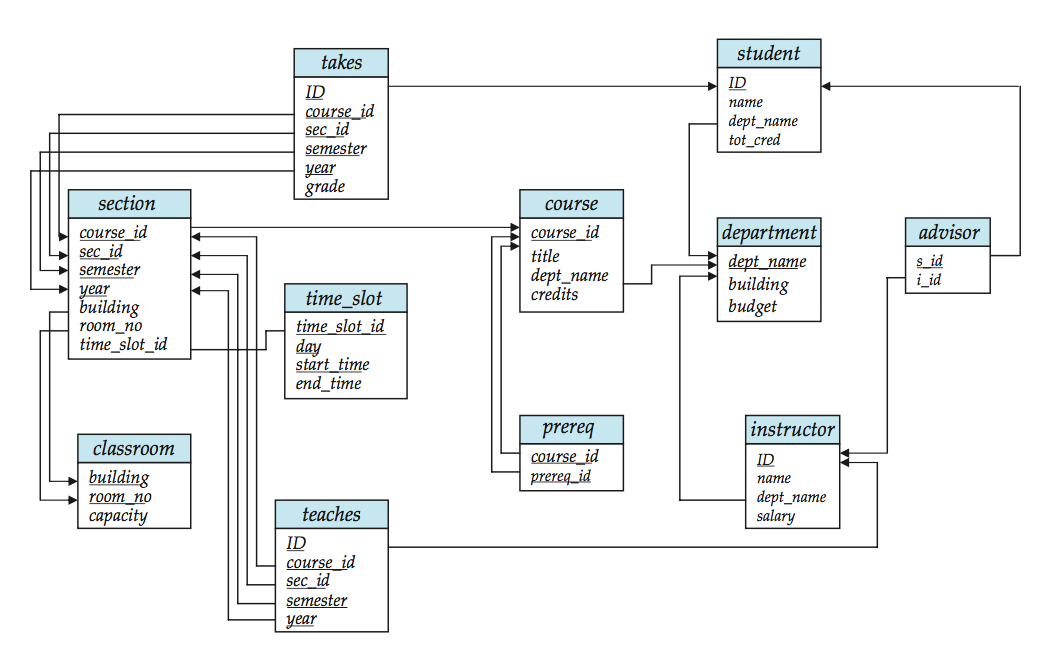
\includegraphics[width=\textwidth]{images/schemadiagram.png}\\
	A database schema diagram representing a ``university''~\cite{dsc}.
\end{center}

\bibliographystyle{alphaurl}
\bibliography{356}


\end{document}
